\chapter[Raven’s Work in Tlingit Ethno-geography]{\vspace{-25pt}Raven’s Work in Tlingit Ethno-geography}

\sethandle{10125/24840}

% \usepackage[
% 	doi=false,
% 	backend=biber,
% 	natbib=true,
% 	style=biblatex-sp-unified,
% 	citestyle=sp-authoryear-comp]{biblatex}
%\usepackage[style=ldc.bst]{biblatex}




% Author last name as it appears in the header
\def\authorlast{Thornton}

% change author in three references below to the actual author name so that this name is unique and matches the \label commands just below and at the end of the chapter
\renewcommand{\beginchapter}{\pageref{thornton-ch-begin}}
\renewcommand{\finishchapter}{\pageref{thornton-ch-end}}
\label{thornton-ch-begin}



\thispagestyle{firststyle}

\chapauth{Thomas Thornton}
\affiliation{University of Alaska Southeast}

\authortoc{Thomas Thornton}



“Raven names,” specifically geographic names by, about, and for the Raven figure of mythic time (de Laguna 1960: 129), comprise a distinct subset of toponyms in Tlingit and other Alaska Native geographic nomenclatures.  The distribution of Raven names is not random or even. Instead Raven names tend to be concentrated in areas of unique geographic abundance, dynamism, and anomaly.  Why is this so? Is it simply because of such sites conjure an elective affinity with Raven’s unique status as shaper and transformer of the world?  Or are there other factors at work?  In this paper, I explore the distribution, relations, and meanings of Raven names in Southeast Alaska and contiguous Canadian Tlingit territories within a fuller anthropological and geographical context than previously available to determine why concentrations of Raven names tend to exist where they do.  In particular I focus upon “Raven’s doings” or “Raven’s work,” as Tlingits sometimes say, as embodied in Raven names and the narratives and that accompany them.

\section{Raven’s Work}
Raven is a namer and landscape transformer in every Alaska Native and Northwest Canada First Nation oral tradition.  As the trickster-demiurge of indigenous mythology he is present at moments of dynamic change on the land, much of which is “Raven’s Work” (Yéil Dzoonáyi, see Table 1, \#20)--as one Tlingit toponym at Alsek River encapsulates—that is, a direct consequence or by-product of his ravenous dwelling.

As I have suggested in \textit{Being and Place among the Tlingit} (2008: 110), Raven is not only subject and source of names on the land, but also cultural model of the Tlingit namer. Raven perceives and negotiates many of same affordances on the land and sea as a human would, including prospects for food, water, fire, shelter, companionship to satisfy his appetites, needs, and interests, as well as hazards that may imperil him.  Yet, as an unprecedentedly endowed bird, he also has additional capacities, including bird’s eye apprehension of the world, the capacity to transform, the ability to communicate across species, and the clever wherewithal to escape danger (by wing or other means).  Many of Raven’s names show these capacities and interests, specifically. For example, Raven informs Bear of a good halibut fishing bank in an area he named “Just on the Edge of the Base of the Kelp” (Geesh K’ishuwanye), indicating both his comprehension of specific (and otherwise hidden) resource patch at the bottom of the sea, and a general principle for locating such places. In this way, Raven and his names are a model for how to apprehend and act on the world, for through his deeds and their legacies he was destined to “[show] all the Tlingit what to do for a living” (Swanton 1909: 83).

The remarkable role of Raven in Tlingit lives is emphasized by the late Lukax.ádi clan leader Austin Hammond (\textit{Daanaawáak}; see Kawaky 1981) in his own inimitable way in the film \textit{Haa Shagóon} (Our Heritage and Destiny).

\begin{quote}It was Raven who showed us how to get our food. Raven knew what was good for us, and taught the Tlingit how to live. Raven exists in our legends and in our lives. Sometimes Raven is powerful and wise, and at other times Raven seems foolish. But always the stories of Raven hold special meaning for us. It was Raven who hung by his beak suspended from the clouds at the time of the Great Flood. It was Raven who taught our people to catch salmon. These are the stories my grandfathers passed on to me. These are the things I’m trying to teach my grandchildren. It is these stories which help guide our people as we live with the land. . . . For Raven taught us, if we live with the land, not against it, the land will take care of us. The land, the river, they hear us!
\end{quote}
\noindent
As linguistic artifacts that describe, distinguish, distill the meanings of places (Thornton 2008), place names are resilient, resonant, and respected sources of Raven’s ever-vibrant relations with Tlingit country, illustrating both the wisdom of living with nature’s vitalism, and the folly of going “against nature,” which is the very definition of taboo, or \textit{ligaas’} in Tlingit (Swanton 1908; de Laguna 1972).

In what follows, I want to expand on the meaning of “Raven’s work” in Tlingit country. Specifically I want to argue that Raven is foundational to the very conceptualization of Tlingit geography because he embodies an integrative set of ideas about the indivisibility of nature/culture and its intrinsic status as: 1) formative and transformative; 2) animistic and dynamistic; 3) relational and contingent; and 4) adaptive and resilient.  As a Trickster-Transformer and world-maker, Raven is special, in his capacity to both stimulate and respond to environmental change.  Raven’s struggles with  and instigations of profound disruptions in the natural order are symptomatic of exigencies of existence in the North Pacific Rim, among the least stable and most dynamic landscapes anywhere in the world.  It is here that we find “Raven’s work.” To illustrate the significance of Raven in Tlingit toponymy, I will analyze several indigenous landscapes in the greater Southeast Alaska region with specific ties to Raven, including 1) the geography of the Great Flood in Tlingit country; and 2) the densely Raven-named and rugged Alsek River-Dry Bay region (see \hl{Map}\todo{Map?}), south of Yakutat, much of which is now part of the grand 24,312,997 acre USA-Canada Kluane/Wrangell-St. Elias/Glacier Bay/ Tatshenshini-Alsek World Heritage Site.

\begin{figure}
	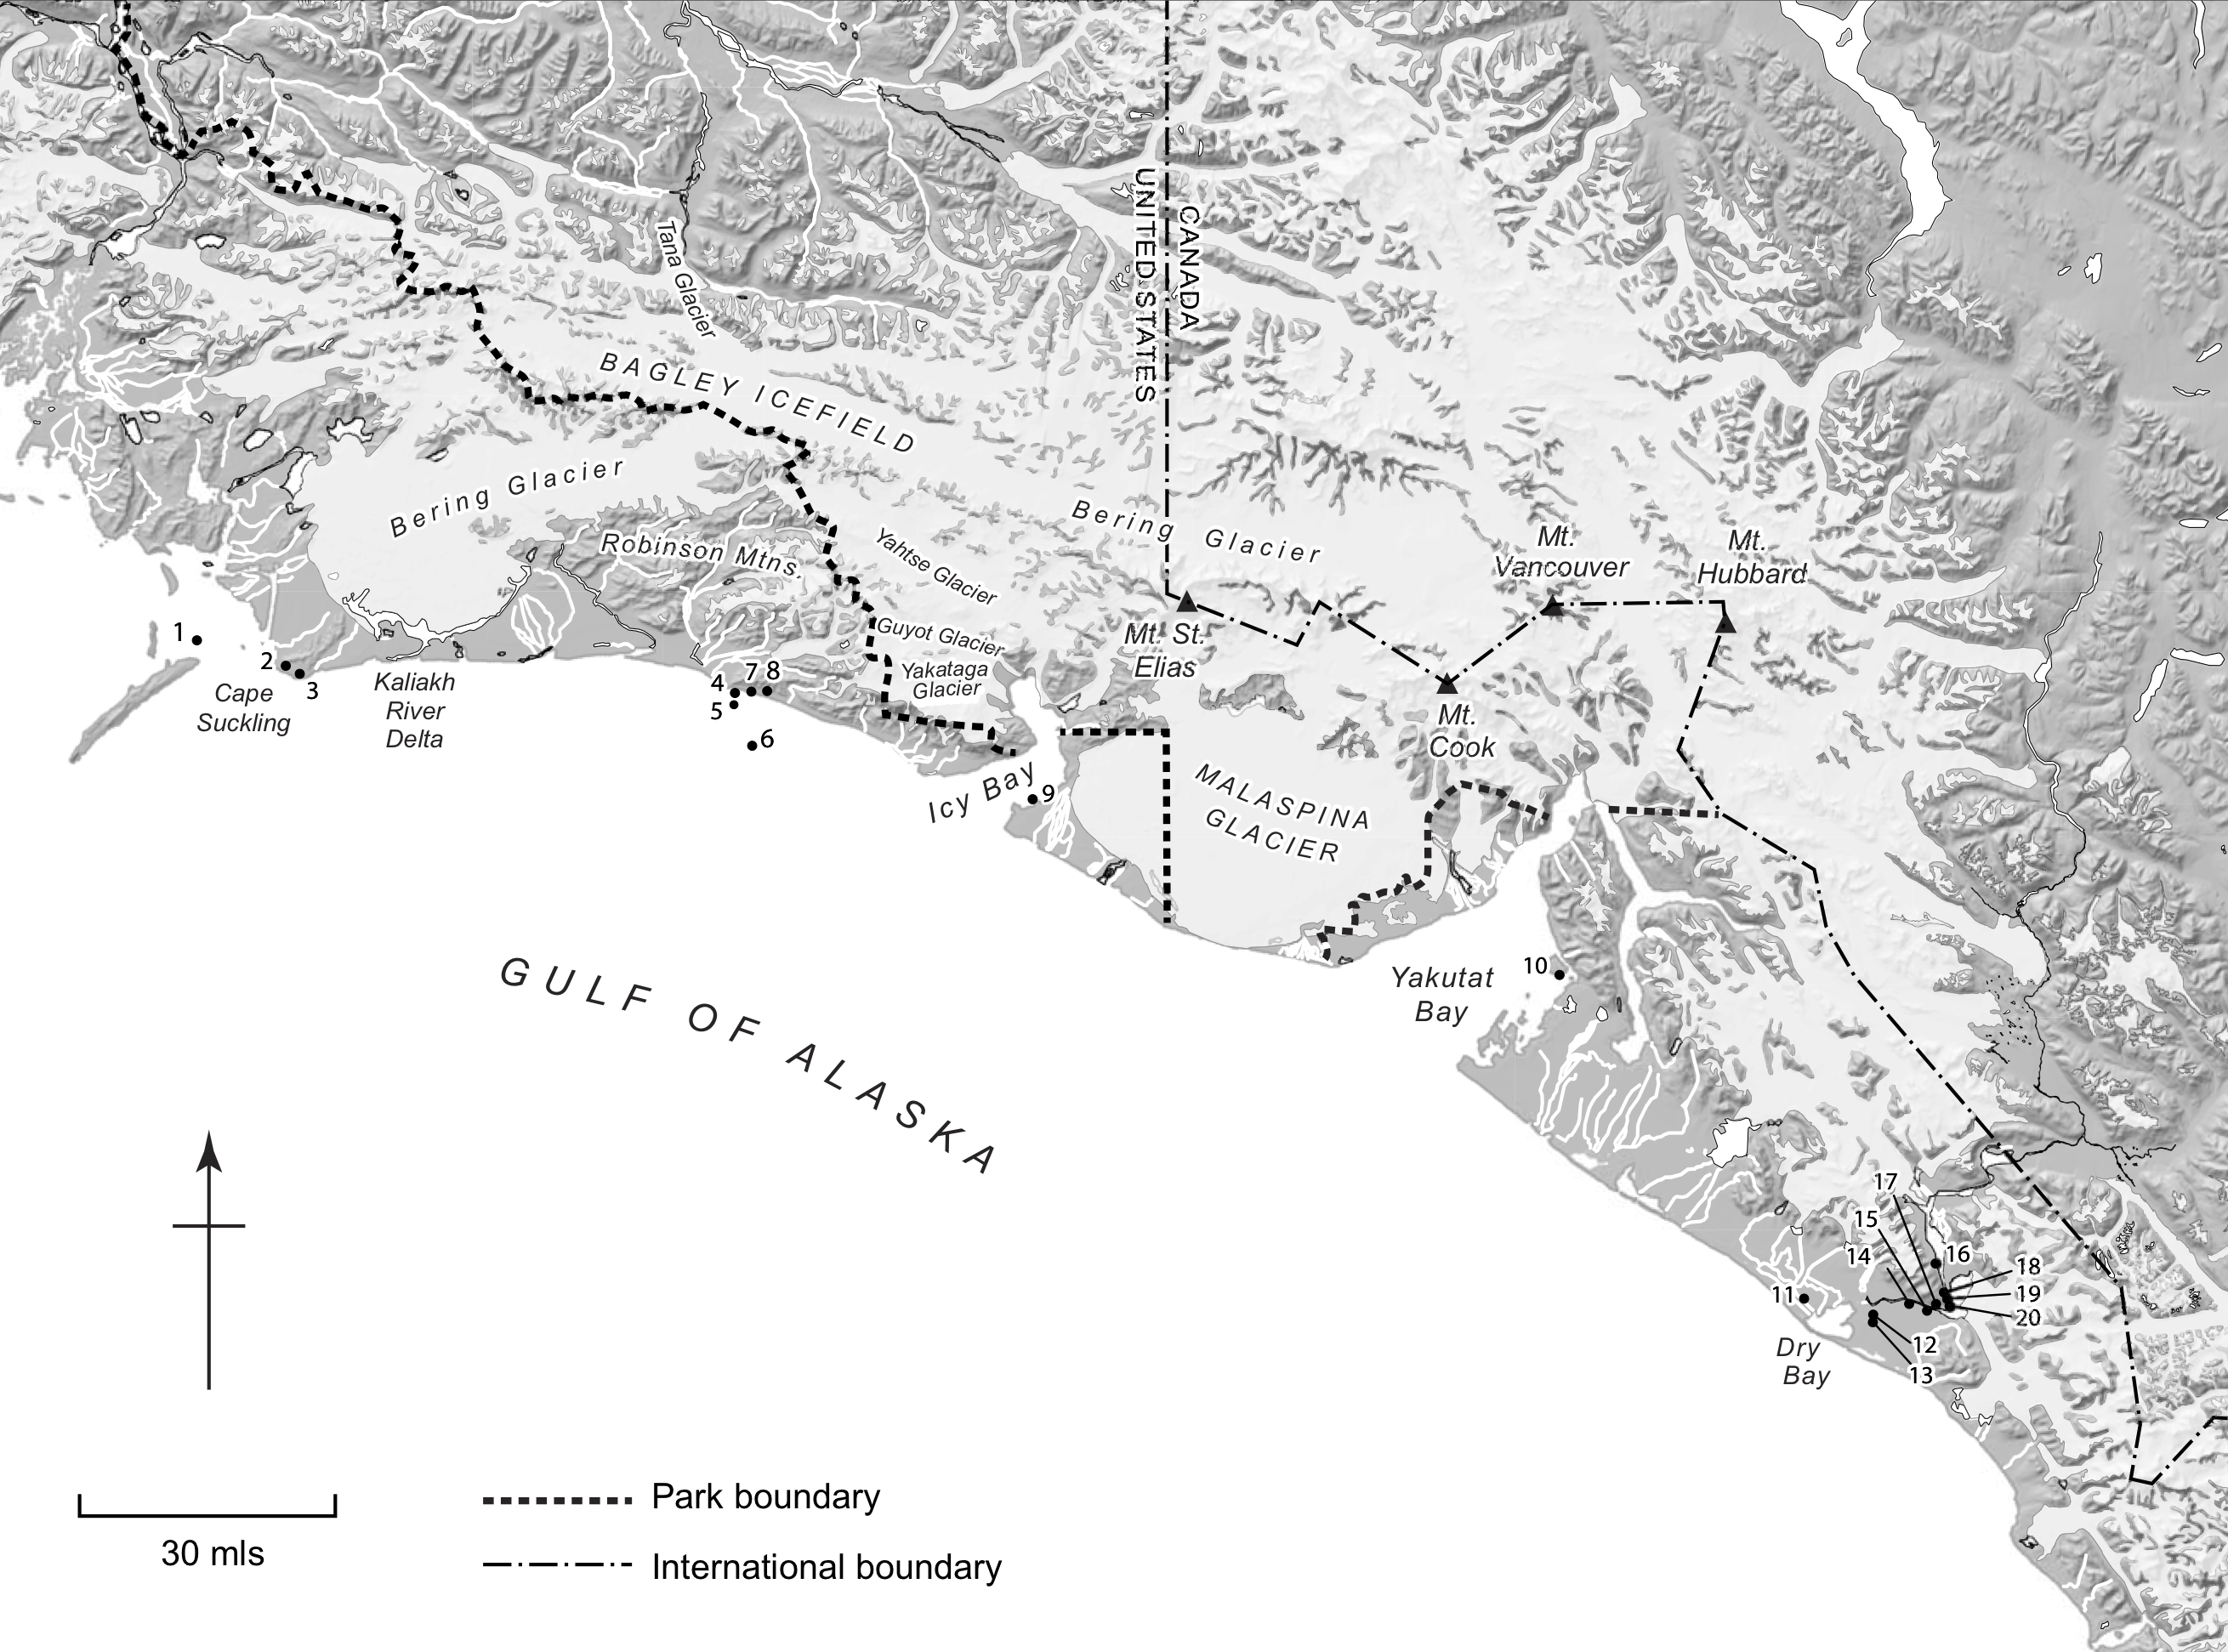
\includegraphics{figures/thornton-map1}
	\caption{\hl{map caption}}
	\label{thornton-map1}	
\end{figure}

\section{The Great Flood}
	Raven’s story begins with the Great Flood, the prototypical environmental change event, usually set at Nass River or elsewhere in Southeast Alaska.  As Chilkat elder David Katzeek tells the story, it was before the great Flood that Raven was born, to a mother who swallowed him after he transformed himself into a small, attractively smooth and shiny stone, at the suggestion of Blue Heron.  Raven was raised by his maternal uncle, who mistreats him, and their conflicts eventually trigger the Great Flood, which manifests not as torrential rainfall, as in the Bible, but rather as a great tide coming in:

\begin{quote}
    [Raven knew] that the tide is really going to come in…So the story goes that after [Raven] put his mother in [a black scoter skin] and he put her out on the water…He let it go [to float as the world flooded].  Let the tide come in.  Then the story goes ... Yéil kaawx̲a awé. Yaa aan xáas’i dei wuditeen.  I love that word [Aan xáas’i], saying that the earth has an outer skin with it way up in the atmosphere where Awu xaligaas, he [Raven] was just hanging above the earth. And nobody knows how long he hung there.  And then the story goes on to say that when the tide—when the water began to recede, was when he let go of that outer skin of the earth and fell all the way down to the waters …no one knows how many days or how long it was for him while he was falling from the outer skin of the earth, that he finally came and landed on \textit{geesh}, on bull kelp, over on this one place [perhaps near Dry Bay].  And when he sat there, up popped the sea otter.  He talked to the sea otter and he asked the sea otter, ‘Can you go all the way to the bottom?’  And that sea otter said ‘Uh huh.  Yes I can.’  ‘Well, then, if you can go all the way to the bottom, bring me some rocks and bring me some sand.’  So the sea otter goes down and brings rocks and sand to Raven.  The story goes when Raven starts throwing---he was throwing rocks out, and as he was throwing rocks all the islands started to form that are here in Alaska.  The sand that he had when he threw it out, it made the Alaska Peninsula all the way on out, the Aleutian Chain... \\

    ... But historically, the reason there are Deisheetaan from the Interior, the reason there are Killer Whales [Dak’laweidí] from the Interior, the reason there are Yanyeidis [and other clans] from the Interior … [is] because of fleeing--because of the great Flood that took place on this earth.  So that’s the story. (Katzeek 2013).
\end{quote}

\noindent
In reordering the Earth through the Flood, Raven remade the land for human habitation, exemplifying the principles of formation and transformation for which he is famous as a Transformer and world-maker. His doings thus became part of Tlingits’, indeed all Alaskan Natives’ heritage and destiny (\textit{haa shagóon} in Tlingit). In one version of the Raven cycle recorded by Swanton (1909: 81) Raven is said to have endured the Flood by turning to rock. After the Flood, it is said that:

\begin{quote}
Raven [Naas Shaak’i Yéil, Raven at the Head of the Nass River] tried to make human beings out of a rock and out of a leaf at the same time, but the rock was slow while the leaf was very quick. Therefore human beings came from the leaf. Then he showed a leaf to the human beings and said, ``You see this leaf. You are to be like it. When it falls off the branch and rots there is nothing left of it.'' That is why there is death in the world. If men had come from the rock there would be no death. Years ago people used to say when they were getting old, "We are unfortunate in not having been made from a rock. Being made from a leaf, we must die.
\end{quote}

By molding people from leaf, Raven recognised the impermanence and mutability of life on earth, the formation and transformation of its beings from seed to leaf and back again.  People may aspire to the immortality of rock (Kan 1989), but life on earth, at least for humans, is governed by change, and change defies the rigidity and permanence of rock, and rewards continued growth, evolution, and renewal of the leaf as a living, adaptive entity. It is important that people did not stand still like rocks in the aftermath of the Flood, but rather redistributed and reorganized themselves, through migration and adaptation, to the new world they faced when the waters receded.

Among the interior Tlingit and Tagish and Southern Tutchone Athapaskans the stories are similar. Elder Annie Ned described to anthropologist Julie Cruikshank (2005: 15) how “Raven, also known as Crow, originally configured the drainages from the interior to coast at the beginning of time, tipping his wings to orient them in the opposite directions; some lakes and rivers now flow north to the Yukon River and hence to the Bering Sea and other pour south to the Gulf of Alaska through the Alsek and Tatshenshini drainage.”  Thus Raven is not only the instigator of the earth-changing Flood, he is the shaper of rivers, the manipulator of tides, and in Tlingit country he is colour of the Pacific Ocean itself, which in the Gulf of Alaska at least, is simply called Yéil T'ooch, Black Raven.  This ocean, too, is Raven’s world, because it is also a result of the great Flood that Raven caused, and which he and his transformed humans had to adapt to when they returned to the coast—him from the sky and they from the mountain stone forts, where they sought refuge. The early naval Lieutenant and ethnographer George T. Emmons (1990: 82) described this mountain refuge geography thusly:

\begin{quote}
... more baffling than petroglyphs and stone carvings are cairns of piled stones to be found on mountains well above timberline, both on the mainland and on offshore islands. They have no relation to the Russian occupation, and are not boundary marks. They are away from any trails or lines of travel, at altitudes of from two to three thousand feet, located on clear stretches, generally on mountain tops. The oldest natives can give no explanation of them, beyond the story that when the great Flood covered the earth, those who survived in canoes floated up and moored their craft here with great bark ropes, the decayed ends of which it is claimed can still be seen.
\end{quote}
\noindent
These mountains “saved a lot of people” the Tlingit elders say (Jack 2013), because they afforded safety and refuge from the Flood, allowing people to survive. And after the Flood, Raven made regular tides in the ocean by manipulating the figure known as Old Woman of the Tides, who controls them, so the aboriginal people could take advantage of the sea’s intertidal bounty. These enduring geographical phenomena, including the ancestral alpine cairns and petrified remains and coastal petroglyphs and other landmarks, often marked by toponyms, remain as testimony to the adaptiveness and resilience of the aboriginal settlers in the region, and to “Raven’s work.”

\section{Raven’s Work in Northern Southeast Alaska and the Alsek River-Dry Bay System}

Between Cape Suckling and Lituya Bay in the Gulf of Alaska, Alaska’s northernmost Tlingit territory, now claimed by clans residing primarily at Yakutat, we find the highest densities of documented Raven names (Table 1).

\begin{table}[!h]
    \centering
		\small
    \begin{tabular}{l | L{3cm} | L{3cm} | L{4cm}}
\textbf{\#} & \textbf{Name} & \textbf{Translation} & \textbf{Location}  \\
\toprule

1&Yéil Xákwdli
&Raven’s Harpoon Line
&Okalee Spit \\

2
&Yéil Katsees
&Raven’s Float
&Between base of Okalee Spit and Cape Suckling \\

3
&Yéil Hít
&Raven’s House
&Cave at Cape Suckling  \\

4
&Yéil X'us.eetí
&Raven’s Footprints
&Cape Yakataga \\

5
&[Yéil ] Tayeesk'*
&Little Adze*
&Cape Yakataga  \\
6
&Yéil (Yeil) T'ooch'
&Black Raven
&Gulf of Alaska (Pacific Ocean) \\

7
&Yakwdeiyí
&Canoe Road
&Inside Cape Yakataga \\
8
&Yéil Naasa.áayi*
&Raven’s Bentwood Box*
&Cape Yakataga area  \\
9
&Geesh K'ishuwanyee
&Place below the End of the Edge of the Base of the Kelp
&Halibut fishing bank, Icy Bay \\

10
&Yéil Áa Daak Wudzigidi Yé
&Place Where Raven Fell Down
&Knight Island, Yakutat Bay \\

11
&Yéil Áx Daak Uwanugu Yé
&Where Raven Scooted Back [Kicking Up the Sand]
&Dunes on Akwe River, Dry Bay \\

12
&Kudatankahídi
&[Raven’s] Repository House
&Dry Bay \\

13&Yáay X’áat’i&Whale Island&Bear Island, Dry Bay \\

14 &Yéil Áa Yoo Akaawajiyi Yé
(Yéil Áx Daak Akawujiyi Yé) &Where Raven’s Feet Worked into the Mud Dragging (the salmon repository or “food canoe”)
&Alsek River \\

15
&Yéil Kínde Akaawatsexi Yé
&Where Raven Trampled [the Ground Packing It] Upward
&Alsek River \\

16
&Yéil Katooli Yé
(Yéilch Uwatuli Yé)
&Hole Raven Bored
&Near Gateway Knob \\

17
&Yéil Yakwdeiyí
&Raven’s Canoe Trail
&Alsek River \\

18
&Yadagwált
&Raven’s Rocks Falling Down
&Gateway Knob area \\

19
&Yéil Áa Ludaawdligoowu Yé
&Place Where Raven Wiped His Beak Off
&Alsek River \\

20
&Yéil Dzoonáyi
&Raven’s Work
&Gateway Knob \\

21
&Yei Wal'ji Héen
&Stream That Breaks Downward
&Where the Alsek River floods \\

22
&Yéil Yakwdeiyí
&Raven’s Canoe Trail
&Cape Fairweather area \\

    \end{tabular}
    \caption{Raven names}
    \label{table1}
\end{table}

The landscape with the highest densities of Raven toponyms by far is the Alsek River-Dry Bay basin, which is perhaps the region’s epicenter for change, dynamism, and Raven’s work.  Here even those toponyms that don’t reference him directly seem to be the result of Raven’s interventions. For example, Bear Island, the major island feature in Dry Bay, is known as Yáay X’áat’i (\#13) Whale Island.  But this is no simple metaphoric reference to the island’s physical resemblance to a Humpback Whale, or metonymic association to the presence of whales around the island.  Rather it is \textit{the} whale that Raven harpooned first at Kayak Island, near Cordova, with his line and float attached (\#s 1 and 2). Raven is then said to have entered the whale through its blowhole, feasted all winter on its blubbery innards, finally beaching his host at the entrance to Dry Bay, where he “wished the Whale to strand on a fine sandy beach” (and thus the Alsek delta is said to be sandy as a result; see de Laguna 1972: 84). The people that lived on the east side of Dry Bay, known as Whale’s Fat (Yáay Taayí) heard Raven calling, and, after initially being scared by the this sound, dragged the whale further ashore and flenzed it, eventually opening a hole big enough for Raven to fly away with his customary “k̲aa!” cry of Trickster triumph, having tricked the people out of some of the whale meat and fat.  Significantly, when the people at Gus'eix̲, the village at Dry Bay, faced a later Flood, caused not by Raven but a local clan’s mistreatment of a seagull, the whale’s “fin,” a marked protrusion on the island, served as a mooring for people to tie their canoes as the flood waters washed the settlement away (de Laguna 1972: 76).\footnote{Today this island, though still recognized for its origins as a whale, carries the Tlingit name Gal'jinoowú (Clam Hand Fort, though its etymology is uncertain, according to de Laguna 1972: 84), perhaps reflecting a major adaptation of the Tlingit and other Northwest Coast peoples: cultivation of clam “forts” or “gardens” (Thornton, et al. 2015), basically engineered beds to stabilize and enhance habitat for these marine invertebrates.  Perhaps such cultivation represents another of Raven’s lessons on how to subsist in a changing world.  Unfortunately, the oral history does not tell us.  }

Raven’s food quest is also evident in his tracks on the west side of Dry Bay, which are produced after he drags in the famous “ark” or food canoe and builds a repository house (\#12, Kudatankahídi), sometimes referred to as Raven’s Party House, variously located at Dry Bay, Cape Yakataga or Cape Suckling.  The food canoe, which in fact also supported kelp-bed edifice to house marine creatures, was heavy and the effort to drag it arduous, these efforts being marked by the place names Yéil Áx̲ Daak̲ Uwanugu Yé (\#11), Where Raven Scooted Back [Kicking Up the Sand] and Yéil Áa Yoo Akaawajiyi Yé  (\#14) or, Yéil Áx̲ Daak̲ Akawujiyi Yé), (Where Raven’s Feet Worked into the Mud Dragging).  According to Yakutat elder Fred White (2001), who spent time with his grandparents at Dry Bay, you can see Raven’s tracks at the sand dunes between Ustay and Akwe rivers, the dunes themselves having resulted from when Raven dragged the canoe to shore, working his feet into the mud, and kicking up sand.  Like Noah’s ark, this great canoe was said to house all the animals we find in the world today.  As de Laguna recorded:

\begin{quote}
    At the Dry Bay (eastern) end of the long, narrow island between these two sloughs, there is a sand dune. On this I was told could still be seen the footprints made when Raven with a cane shaped like a devilfish tentacle drew ashore an ``ark'' filled with all kinds of food animals. Canoe Prow House of the [L’uknax̲.ádi clan] refers to the enclosed prow of this canoe, and the [L’uknax.ádi] use a dance paddle shaped like the cane. The point, 'Atuqka [?] [Evidently the “fin” used to moor the canoes in the abovementioned flood], was "a place just like the prow of a canoe...”
\end{quote}

Bert Adams (1998), a L’uknax̲.ádi clan elder, adds: “When he pulled the ark ashore, the birds were released and that is why we have birds in the world today.  As he pulled the ark from the ocean he left his foot prints in the sand hills along the Akwe River and that is where Gus'eix̲ [village] is. This goes along with the story that the Lukaax̲.ádi [another clan] people were the earliest people in the Dry Bay area and initially built their house in Gus'eix̲. When the L’uknx̲x.ádi people came from southeast they eventually took over Gus'eix̲ and probably changed the name to Digginna hit [Deikinaa Hít], Far Out House.”

Bert Adams, Fred White and others (see de Laguna 1972), also agree it was at Alsek River-Dry Bay where Raven opened The Box of Daylight he stole form his grandfather at Nass River (de Laguna 1972: 84), and in doing so, not only released the sun, the moon and the stars into the cosmos, but frightened everything else—even the rocks and the mountains---off the face of the land from Dry Bay up to Ocean Cape, leaving only sandy forelands.

\begin{quote}
Raven also lured ashore the first king salmon in Dry Bay. The mountain down which Raven was thrown in a box, is above the Akwe River. Near the second glacier ascending the Alsek, Raven threw away his wife's basket and a big king salmon. The cave, or house of stone [Yéil Ta Hít?], in which Raven lived is southeast of Lituya Bay; it is [in] the mountain he slashed [Yéil Nées' Akawlishaa, Raven Ate Sea Urchin, perhaps Mount Crillon or Mount La Pérouse] when angry at Echo [for imitating his loud slurping sounds, eating sea urchins (see also de Laguna 1972: 93)].  In this area, Raven obtained the first plants and trees from the Sea Otters [after the Great Flood, referenced above]. There is also another of his landing places near Cape Fairweather or Lituya Bay. It is in this area where we can see how the surface of the land was shaped in primordial time (Adams 1998).
\end{quote}
\noindent
Thus, Raven’s Alsek River-Dry Bay landscape is not only the source of all creatures in the world, but the source of the world itself, and the place where the entire planetary system was released to support life on earth.

Animism and dynamism in the land are reflected in the Alsek River itself, and its major tributary, the Tatshenshini, which were both said to possess powerful spirits and animate geographic features and constituted lucrative trade routes and perilous passages. Trade routes linked the coast and Interior Tlingit and Athabaskan communities, and also lead to the wealthy Chilkat and Chilkoot Tlingit tribes at Haines (Deishu, End of the Trail) and Klukwan (Tlákw.aan, Eternal Village) (De Laguna 1972; Thornton 2011, 2012). Deieenaak’w, The Sitka elder who recorded much Tlingit oral history for Swanton in 1904 (Swanton 1909), emphasized the living spirit and animistic qualities of the glaciers in this area: “In one place Alsek River runs under a glacier. People can pass beneath in their canoes, but, if anyone speaks while they are under it, the glacier comes down on them. They say that in those [early] times, this glacier was like animal and could hear what was said to it.” The dangers, including recurring ice bridges, blockages, and flooding are well catalogued by Natives and non-Natives alike (see de Laguna 1972: 87), and summarized by Cruikshank (2005: 236; see also de Laguna 1972: 885-90):

\begin{quote}
Danger points reported by all river travelers were two canyons, each formed by a rock wall facing an actively calving glacier (see conventional 9). At the first, about 30 kilometres upriver from the mouth, an expanded Alsek Glacier formed a vertical wall of ice some sixty metres high, stretching for more than six kilometres and interrupted only by “Gateway Knob,” a tall nunatak or promontory from which rocks the size of golf balls rained down. It was here that an ice bridge formed periodically.  Sometimes a lake, subject to outbursts [i.e., flooding], formed just below. Tlingit narrators attributed Gateway Knob’s formation to the travelling world-maker, Raven, who distributed geophysical features at the beginning of time. They commented on Raven’s wife’s dismay whenever she passed beneath this knob’s jutting rock face, lest she be killed, and Raven’s modest reassurances that rocks would not touch the boat unless some passenger was fated to die.
\end{quote}

"That's where the rocks fall all around,” one of de Laguna’s (1972: 87) informants remarked, “and they call it Yel tsunayI [Yéil Dzoonáyi, Raven's Work]. When my father was going up to Tinx kayani [Tínx Kayaaní, Bearberry/Kinnikinnick Leaves, near Sediment Creek on the Tatshenshini River], it [the golf ball sized rocks] touched his boat. That same summer they drowned."  Even today, more than an half century after de Laguna’s last major fieldwork, these stories still resonate, enlivening the landscape and enlightening people as to how to engage its potency.  These rules of engagement, entailed by Raven’s instigations, but evolving through subsequent relations with human and other-than-human beings remain relevant and contingent for success in adaptation and resilience in this dynamic, ever-changing landscape. Thus, songs and sayings people recited as they passed vulnerably under the Alsek’s ice bridges, active glaciers, and shedding rock walls-- Yéil Dzoonáyi— are remembered and performed at potlaches and other appropriate contexts, rendering Raven’s work and its entailing events as sacred \textit{shagóon} or chronotopes,, places in a community’s geography where time and space are forever fused as sacred heritage and destiny (see Bakhtin, cited in Thornton 2008: 17).

\section{Conclusion: The Resonance of Raven Landscapes from the Pleistocene to the Anthropocene}

Raven names form not only a genre of geographic nomenclature but mark exceptional, dynamic and anomalous environments throughout Tlingit country and beyond.  I have focused particularly on well documented Raven geographies in mythic time (the Great Flood) and the contemporary late Holocene in northern Southeast Alaska.  While I have highlighted the dynamic far northern Dry Bay-Alsek River frontiers of the Tlingit settlement, other unique and potent parts of their territory exhibit similarly evocative Raven names and evidence of his “work” on the land,  if not in the same rich concentration: Kootznahoo Inlet inside Angoon, with its strong reversing tidal falls (Yéil Eeyí ,Raven’s Tidal Current), Keku Straits and Saginaw Bay areas near Kake (e.g., Yéil G̲áachk'u, Raven’s Little Mat, a flat-topped island landmark in the Keku Islands where Raven laid a mat of plants, and Yéil Kawóot, Raven’s Beads, a unique limestone bed of fossil crinoids that Raven once used to fashion a necklace for his wife); Peril Straits above Sitka with its narrow passes and forceful currents (e.g., Yéilch Wóoshdáx̲ Wulixidi Yé, Place where Raven Broke Through, by creating a passage with his paddle); and Upper Lynn Canal near Haines with its dramatic mountain canyons and rocky shores (e.g., Yéil Háatl'i, Raven’s Excrement, a rocky shore near Battery Point, below Haines, or Yéil Áx' Sh Wulg̲eig̲i Yé, Place Where Raven Swung, in a mountain valley) (see Thornton 2012).

As the legends recount, Raven had to steal the various elements that comprise the world—the earth, the moon, the stars, freshwater, fire--and, after enlightening and enlivening the world, he embarked on his quest to gather together those resources necessary to sustain a life: freshwater, wood and other materials for fire and manufacture, medicines, and various foods. His descendants still pursue this quest and follow the trails he has inscribed in the landscape. People hunt, fish, and gather in the vicinity of X’as’tuhéen ([Raven’s] Driblet Creek, in Excursion Inlet, Near Hoonah), created by the drops that spilled from Raven’s mouth as he flew away from Petrel after stealing the latter’s spring water (at Hazy Islands, southwest of Kuiu Island); collect intertidal resources at Skanáx (Noisy Beach, in Saginaw Bay, where Raven found the squirting bivalves cacophonous); land their boats at Yéil Kiji Yakwdeiyí (Raven’s Wings Boat Road, on the Khaz Peninsula, near Sitka), where he quieted the sea to create a smooth trail amid the rocks and swells so he could safely land his canoe; and net fish in the vicinity of Yéil G̲eiwú (Raven’s Web or Fishnet, at Gut Bay, a premier sockeye salmon stream on Eastern Baranof Island used by primarily by Kake Tlingits), now petrified in stone above the tide line, the webbing still visible (de Laguna 1960). These are just a few of the ways that Raven’s work continues to shape peoples understandings and responses to the land throughout Tlingit country.

Given his special association with unique, dynamic and transforming landscapes, it is no accident that so many of Raven’s acts in Tlingit country can be traced, in one form or another, to the greater Dry Bay-Alsek River area.  This landscape is one of the richest and most remarkable anywhere in the world in terms of its topographic and microclimatic variation, active tectonic, glacial and fluvial processes, abundance of fish, wildlife and edible plants, as well as sheer grandeur.  From the standpoint of human being making a living, it also has all of the affordances (see Thornton 2011) to sustain and endanger life in all of its vicissitudes and vitality. At the same time, this landscape constitutes a palimpsest or meshwork (Ingold 2000) of lines of intersection, interrelation, and interanimation among its constituent beings and the forces that have shaped their dwelling over the longue durée.  Among the lines of intersection are the “hydronymic districts”---a concept coined by Jim Kari in his pioneering studies of Athabaskan place names---which manifest in the lower and middle Alsek and Tatshenshini rivers between Athabaskan and Tlingit toponyms.  Other lines relate prehistory to present history, interior-coast trade, travel, and migration, and animate relations between people, land and sea.  Raven is foundational to all these connections and we would be wise to promote further understanding of his toponymic districts and their associations to better understand, value, and conserve this World Heritage site.  For it was here that Raven formed and transformed the land itself, spawned earth’s systems by opening the Box of Daylight, and showed the people how to navigate and negotiate the exigencies of life, to make their living with nature, not against it, and to adapt and survive in this complex, ever-changing world.

In the end, then, Raven names embody all that this Trickster-Transformer-Worldmaker has represented from his mythic beginnings: a set of powerful, contingent, collaborative and conflicting appetites and forces that make physical and social existence possible but also a continuous drama and struggle. In this sense, as I have argued elsewhere, Raven’s unruly foibles and inscriptions on the land constitute a good model for how to understand not only the Pleistocene and the Holocene, but also what contemporary scientists have termed “The Anthropocene,” a new geologic epoch in which human activities are now impacting most profoundly on the very earth systems that we rely on to sustain us (cf. Crutzen and Stoermer 2000; Thornton and Thornton 2015).  Pessimistic prognosticators see a great reckoning ahead in this new epoch, payback for the havoc humans have wreaked on the planet in the industrial age, while optimists see opportunities for humans to embrace their dominance and engineer a better world.  Raven reminds us that both visions are flawed, and anthropocentric.  The Great Flood, darkness, famine, and other disasters have all been visited on earth before, with many winners and losers, but the people survived, rock-like on the mountain tops. And when the topography and ecology changed, they adapted, flexibly and resiliently, renewing themselves, like leaves.  At the same time, as Raven also shows us, hubris and the aspiration to engineer the earth to our selfish ends have always been with us. But for us, as for Raven, things rarely work out as planned, and when we insult or push earth systems too far (as in the Tlingit concept of taboo, \textit{ligaas’}, “against nature”), there are often unanticipated consequences: other living beings, including the rocks, the waters, and the glaciers, may push back, putting humans in jeopardy.  Thus, humility, awareness and attentiveness to earth systems and other-than-human beings, and, finally, preparation for change and contingency are in order if we are to survive the Anthropocene.  This is but one of many lessons implicit in Raven’s integrated toponymy and topography at Dry Bay-Alsek River and elsewhere in Alaska and beyond, where we find Raven’s work. Before there was the Anthropocene there was the “Ravencene,” and it was bigger, more dramatic, and more all-encompassing than its new anthropocentric counterpart. More importantly, it will always be with us in one form or another.


\refheading

\begin{hang}
Adams, Bert. 1998. Interview and Stories of Dry Bay, Alaska, Project Jukebox, University of Alaska, Fairbanks. Accessed August 2015. \url{http://jukebox.uaf.edu/drybay/htm/stories.htm}

Cruikshank, Julie. 2005. \textit{Do Glaciers Listen? Local Knowledge, Colonial Encounters and Social Imagination}. Vancouver: University of British Columbia Press.

Crutzen, Paul J. \& Eugene F. Stoermer.  2000. The Anthropocene. \textit{Global Change Newsletter} 41. 17–18.

De Laguna, Frederica. 1960. \textit{The Story of a Tlingit Community: A Problem in the Relationship between Archeological, Ethnological, and Historical Methods}. Bureau of American Ethnology, Bulletin 172. Washington DC: US Government Printing Office.

De Laguna, Frederica. 1972. \textit{Under Mount Saint Elias: The History and Culture of the Yakutat Tlingit}. 3 vols. Washington, DC: Smithsonian Institution Press.

Ingold, Tim . 2000. \textit{The Perception of the Environment: Essays in Livelihood, Dwelling, and Skill}. London: Routledge.

Jack, Mabel. 2013.  Interview with Thomas F. Thornton for Alpine Cairn project, National Science Foundation. Angoon, Alaska, July 24. Transcript in Thornton’s possession.

Kan, Sergei. 1989. \textit{Symbolic Immortality: The Tlingit Potlatch of the Nineteenth Century}. Washington, DC: Smithsonian Institution Press.

Kari, James. 1987. Some Principles of Alaska Athabaskan Toponymic Knowledge. In Mary R. Key \& Henry Koenigswald (eds.), \textit{General and Amerindian Ethnolinguistics: In Remembrance of Stanley Newman}, 129–49. Berlin: Mouton de Gruyter.

Kari, James. 1996. A Preliminary View of Hydronymic Districts in Northern Athabaskan Prehistory. \textit{Names}  44(4). 253-71.

Katzeek, David. 2013. Interview with Thomas F. Thornton for Alpine Cairn project, National Science Foundation. Juneau, Alaska, July 22.

Kawaky, Joseph (producer). 1981. \textit{Haa Shagóon}. Film presented by Chilkoot Indian Association. Juneau, AK: Sealaska Heritage Foundation

Swanton, John R. 1908. Tlingit.  \todo{incomplete reference?}

Swanton, John R.. 1909. \textit{Tlingit Myths and Texts}. Bureau of American Ethnology, Bulletin 39. Washington, DC: Government Printing Office.

Thornton, Thomas F.   2008.	\textit{Being and Place among the Tlingit}.  Seattle: University of Washington Press.

Thornton, Thomas F. 2011.  Language and landscape among the Tlingit. In   David M. Mark, Andrew G. Turk, Niclas Burenhult \& David Stea (eds.), \textit{Landscape in Language: Transdisciplinary Perspectives}, 275-89. Amsterdam and Philadelphia: John Benjamins Publishing.

Thornton, Thomas F. (ed.). 2012.	\textit{Haa Léelk'w Has Aaní Saax'ú: Our Grandparents’ Names on the Land}. Seattle and Juneau: University of Washington Press and Sealaska Heritage Institute.

Thornton, Thomas F., Douglas Deur \& Herman Kitka Sr. 2015. Cultivation of Salmon and Other Marine Resources on the Northwest Coast of North America. \textit{Human Ecology} 43(2). 189-199.

Thornton, Thomas F. \& Patricia M. Thornton. 2015. The Mutable, the Mythical, and the Managerial: Raven Narratives and the Anthropocene. \textit{Environment and Society: Advances in Research} 6(1). 66-86.

White, Fred. 2001. Interview on Dry Bay, Alaska, Project Jukebox, University of Alaska, Fairbanks. Accessed August 2014. \url{http://jukebox.uaf.edu/drybay/htm/tape10.htm}

\end{hang}


\orcidfooter{Thomas Thornton}{tthornto@alaska.edu}{}
\label{thornton-ch-end}
